\chapter[DFT Reference DB]{Results: DFT Reference Database}
\label{chap:resultsdftdb}


\begin{changemargin}{1.0cm}{1.0cm}
\abstractpreamble{The key parameters required for Quantum Espresso are converged and selected in preparation for the upcoming calculations.  A set of atom configurations for \acrshort{fcc} crystals are created and \acrshort{dft} is used to computer the energy, forces and stresses on these crystals.\\ \\ \acrshort{fcc} iron does not exist at normal room temperature and pressure, without the addition of a austenite stabiliser.  A set of \acrshort{dft} calculations are used to compute the bulk modulus, lattice parameter and cohesive energy of pure Fe \acrshort{fcc}.  Ruthenium has a \acrshort{hcp} structure and similarly \acrshort{dft} calculations are used to compute bulk properties of \acrshort{fcc} Ruthenium.\\\\The database of bulk properties and atom configuration are used in chapter \ref{chap:resultsfitting} to derive potentials for both Fe-Pd and Fe-Ru as well as for the pure elements.}  
\end{changemargin}







\section{Introduction}

While computer technology has advanced almost in accordance with Moore's law, the calculations involved to approximately simulate simple structures with Quantum Mechanics are barely accessible.  Ideally, crystal structures with several hundred atoms, containing Fe, Cr, and Ni with Ru or Pd would have been used to derive a potential describing all combinations of elements.  

The computer used did not have the resources required for such calculations, and so the model was simplified to either Fe-Pd or Fe-Ru.  The ferromagentism and antiferromagnetism of Fe and Cr were explored using collinear spin \acrshort{dft} calculations.  Due to the improvement in modelling given by including magnetism, all calculations for the reference database were collinear spin.

A number of computer codes were developed to automate processes.  QECONVERGE creates input files and calls PWscf to converge parameters used in this work (section \ref{code:qeconverge}).  QEEOS also creates input files for PWscf but computes bulk properties such as the equation of state, bulk modulus and elastic constants (section(\ref{code:qeeos}).


%%%%%%%%%%%%%%%%%%%%%%%%%%%%%%%%%%%%%%%%%%%%%%%%%%%%%%%%%%%%%%%%%%%%%%%%%%%%%%%%%%%%%%%%%%%%%%%%%%%%%%%%%%
%%
%%  QECONVERGE
%%  
%%%%%%%%%%%%%%%%%%%%%%%%%%%%%%%%%%%%%%%%%%%%%%%%%%%%%%%%%%%%%%%%%%%%%%%%%%%%%%%%%%%%%%%%%%%%%%%%%%%%%%%%%%



\FloatBarrier
\section{QECONVERGE Python Code}
\label{code:qeconverge}

\subsection{Purpose of Code}

The process of converging cutoff parameters is one that may be automated.  A program was developed in Python to automatically converge the ecutwfc and ecutrho values within a specified threshold.

The program reads an input file into memory, and this contains the settings for the convergence run.  A template PWscf input file is also loaded, and this will detail any required PWscf settings, such as the pseudopotentials, atom species and so on.  

Once these files have been loaded, the first stage of the program runs to determine the ecutwfc and ecutrho values that are within the force and energy convergence thresholds provided by the user.  The program creates a crystal based on the settings, for example an FCC, BCC or SC crystal supercell.  The exact atomic positions are likely to be the optimal, relaxed, positions and so the overall forces on each atom will be zero.  The program randomly varies the atomic positions, and this results in a configuration with forces between the atoms.

The wfc value starts with the user defined ecutwfc starting value, and this is increased until the change in energy and force both converge to within the specified thresholds.  The ecutrho value is increased simultaneously, and is four times the ecutwfc value.  In the second stage, the ecutrho value is decreased and the ecutwfc value is fixed while the energy and force remain within their respective convergence thresholds.  Finally, the program attempts to decrease the ecutwfc value further.

Following the energy and charge density cutoff, the program then runs a number of calculations in order to produce a collection of colour density plots of energy cutoff vs density cutoff, plotting the convergence of total energy and total force.  This allows the user to visualise the convergence surface and select cutoff values manually, if desired.

The final part of the program is to help the user decide upon degauss and k-point values.  The converged ecutwfc and ecutrho values from the first part of the code are used, and the k-point start, end and increment amounts are set by the user, as is a list of smearing degauss values.  2D colour plots of force and energy convergence as smearing changes and k-point value changes are prepared and saved so the user may study these to determine the best combination for their application.

The randomised atom positions use a seed that may be set in the input file.  This means that, although they are pseudo-rng generated, they are repeatable given the same random seed.  Every successful PWscf calculation is logged and saved.  If the program runs multiple times, the cached output files are used rather than recalculating every input file.


\subsection{Source Code and Instructions}

The source code and instructions on how to use the program are available to download from GitHub.

https://github.com/BenPalmer1983/qeconverge





%%%%%%%%%%%%%%%%%%%%%%%%%%%%%%%%%%%%%%%%%%%%%%%%%%%%%%%%%%%%%%%%%%%%%%%%%%%%%%%%%%%%%%%%%%%%%%%%%%%%%%%%%%
%%
%%  Convergence Results
%%  
%%%%%%%%%%%%%%%%%%%%%%%%%%%%%%%%%%%%%%%%%%%%%%%%%%%%%%%%%%%%%%%%%%%%%%%%%%%%%%%%%%%%%%%%%%%%%%%%%%%%%%%%%%

\FloatBarrier
\section[DFT Parameter Convergence]{Convergence of Key DFT Settings and Testing}

\subsection{Pseudopotential}

Prior to generating a database of atom configurations, calculated forces, stresses and energies, key \acrshort{dft} settings needed to be selected and tested.  The Python code QECONVERGE was written then used to converge the ecutwfc, ecutrho, k-points and degauss smearing values for each of the pseudopotentials required.
  
As discussed in previously (section \ref{section:backgroundpseudopotentials}) the \acrshort{gga} type pseudo-potential more reliably calculated the bulk properties of a material when compared to \acrshort{lda}/\acrshort{lsda}, and a copy of the earlier table is given in table \ref{table:ggavslsdacopy}.

\FloatBarrier 
\begin{table}[h]
\begin{center}
\renewcommand{\arraystretch}{1.2}
\begin{tabular}{c c c c}
\hline\hline
Pseudo-potential & Element & a/angs & $B_0$/GPa \\
\hline\hline
Experimental    & Na      & 4.29\cite{periodictablena} & 6.3\cite{periodictablena} \\
Na.pz-spn-kjpaw\_psl.1.0.0 & Na & 4.06 & 8.72 \\
Na.pbe-spn-kjpaw\_psl.1.0.0 & Na & 4.20 & 7.67 \\
Na.pbesol-spn-kjpaw\_psl.1.0.0 & Na & 4.17 & 7.50 \\
Experimental    & Al      & 4.05\cite{periodictableal} & 76\cite{periodictableal} \\
Al.pz-nl-kjpaw\_psl.1.0.0 & Al & 3.98 & 78.6 \\
Al.pz-n-kjpaw\_psl.1.0.0 & Al & 3.98 & 78.6 \\
Al.pbe-nl-kjpaw\_psl.1.0.0 & Al & 4.04 & 91.3 \\
Al.pbe-n-kjpaw\_psl.1.0.0 & Al & 4.04 & 75.0 \\
Al.pbesol-nl-kjpaw\_psl.1.0.0 & Al & 4.01 & 87.7 \\
Al.pbesol-n-kjpaw\_psl.1.0.0 & Al & 4.01 & 79.0 \\
\hline\hline
\end{tabular}
\end{center}
\caption{Experimental vs \acrshort{lsda} vs \acrshort{gga} - the \acrshort{dft} values were computed with a PWscf\cite{quantumespresso} using a 2x2x2 cell, 7x7x7 kpoints and ecutwfc=50}
\label{table:ggavslsdacopy}
\end{table}

\FloatBarrier 

The following pseudo-potential files were used for each element:

\begin{itemize}
\item Aluminium: a plane wave GGA potential Pd.pbe-spn-kjpaw\_psl.1.0.0.UPF
\item Chromium: a plane wave GGA potential Cr.pbe-spn-kjpaw\_psl.1.0.0.UPF
\item Iron: a plane wave GGA potential Fe.pbe-spn-kjpaw\_psl.1.0.0.UPF 
\item Palladium: a plane wave GGA potential Pd.pbe-spn-kjpaw\_psl.1.0.0.UPF
\item Ruthenium: a plane wave GGA potential Ru.pbe-spn-kjpaw\_psl.1.0.0.UPF
\end{itemize}

For each pseudo-potential, the ecutwfc, ecutrho and kpoint and degauss settings were converged.  Ideally, the k-points settings would have been increased, but doing so would have been prohibitive due to the amount of time taken to perform each calculation.

By the time calculations were being executed for a 32 atom supercell, one node of 20 processor cores would run for several days up to a week or more, requiring the calculation to be submitted to the job queue multiple times.  Al is also considered in the results section, as it is a simpler atom to run trial calculations with, and to compare to experimental results.











\FloatBarrier
\subsection{Collinear Spin Calculations}

The relaxed crystal lattice parameters were calculated for Fe, Cr, Pd and Ru.  Cr will not be used in either the Fe-Pd or Fe-Ru fitting calculations.  However, there is a large increase in computation time between non-spin and collinear spin calculations.  The ferromagnetic structure of BCC Fe, antiferromagnetic structure of FCC Fe and BCC Cr were investigated. 

\FloatBarrier
\begin{figure}[h]
\begin{center}
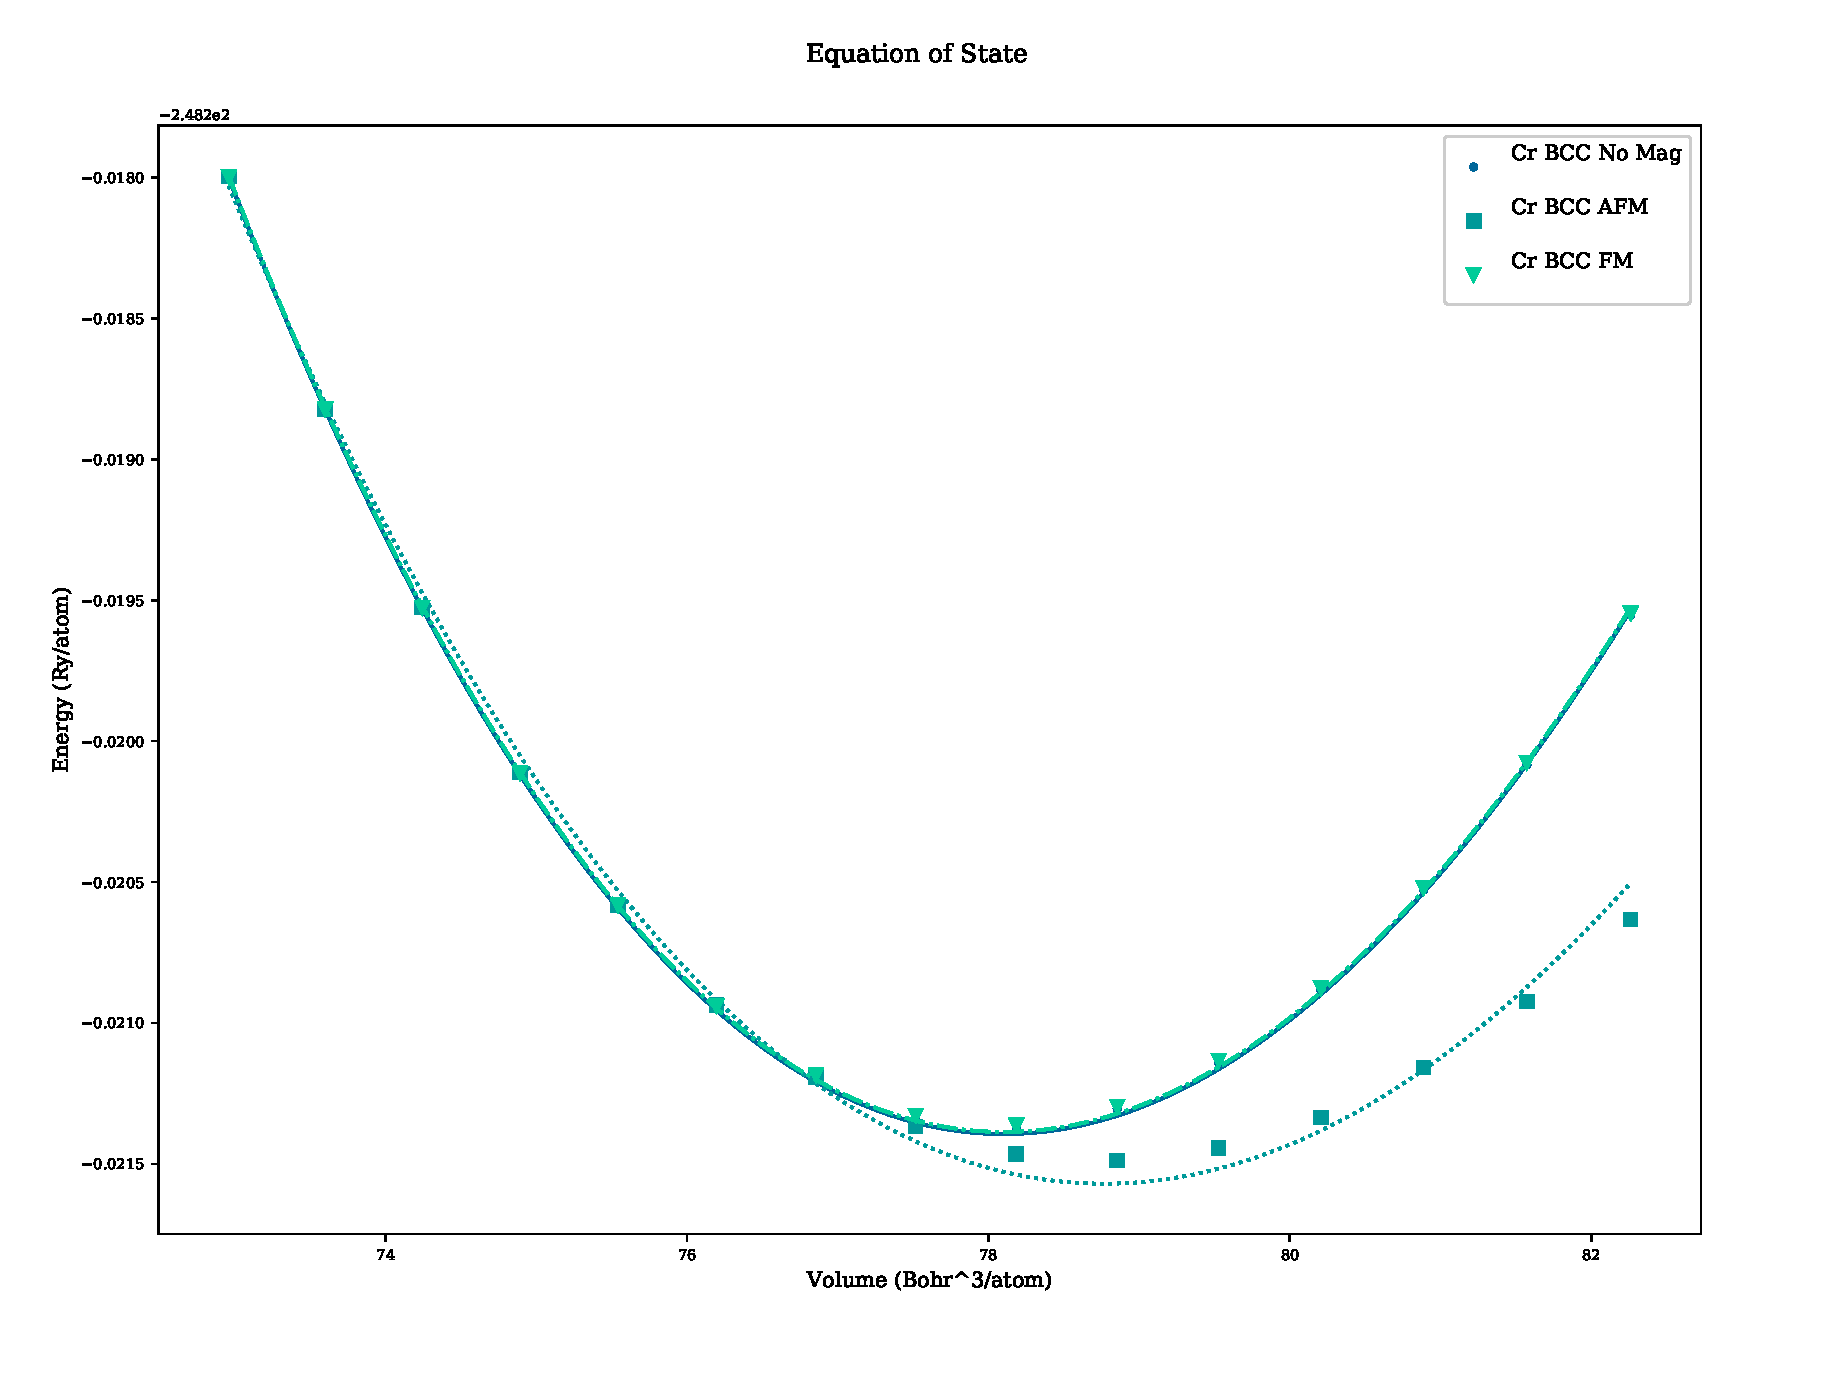
\includegraphics[scale=0.45]{chapters/results_dft_reference_db/qeeos_plots/cr-mag/eos.eps}
\caption{Equation of state fit through data points for Chromium BCC with no magnetism, ferromagnetic and antiferromagnetic configurations}
\label{fig:chromiumeos}
\end{center}
\end{figure}


\FloatBarrier
\begin{table}[h]
\begin{center}
\renewcommand{\arraystretch}{1.2}
\begin{tabular}{c c c c c c}
\hline\hline
Description & $A_0$ (ang) & $V_0$ (bohr3) & $B_0$ (GPA) & $E_0$ (Ry) (DFT Only) \\
\hline\hline
Exp. & 2.91 & 83.23 & 160 & - \\
AFM & 2.86 & 78.77 & 217 & -248.2216 \\
FM & 2.85 & 78.10 & 267 & -248.2214 \\
No Mag & 2.85 & 78.102 & 267 & -248.2214 \\
\hline\hline
\end{tabular}
\end{center}
\caption{Chromium properties with and without collinear spin}
\label{table:crproperties}
\end{table}
\FloatBarrier

The equation of state was calculated for Chromium BCC in three ways: (1) with magnetism switched off, (2) atoms set in a ferromagnetic configuration (collinear, all in the same direction), (3) atoms set in an antiferromagnetic configuration (collinear, atoms in the same cell with spin in opposing directions).  

The DFT calculated values for the bulk modulus were larger than expected, but the antiferromagnetic calculation was much closer to the experimental value (table \ref{table:crproperties}).  The $E_0$ values do not reflect the actual energies, but show the relative calculated values.  The antiferromagnetic configuration gives the lowest, optimum, energy (fig. \ref{fig:chromiumeos}).

\FloatBarrier
\begin{figure}[h]
\begin{center}
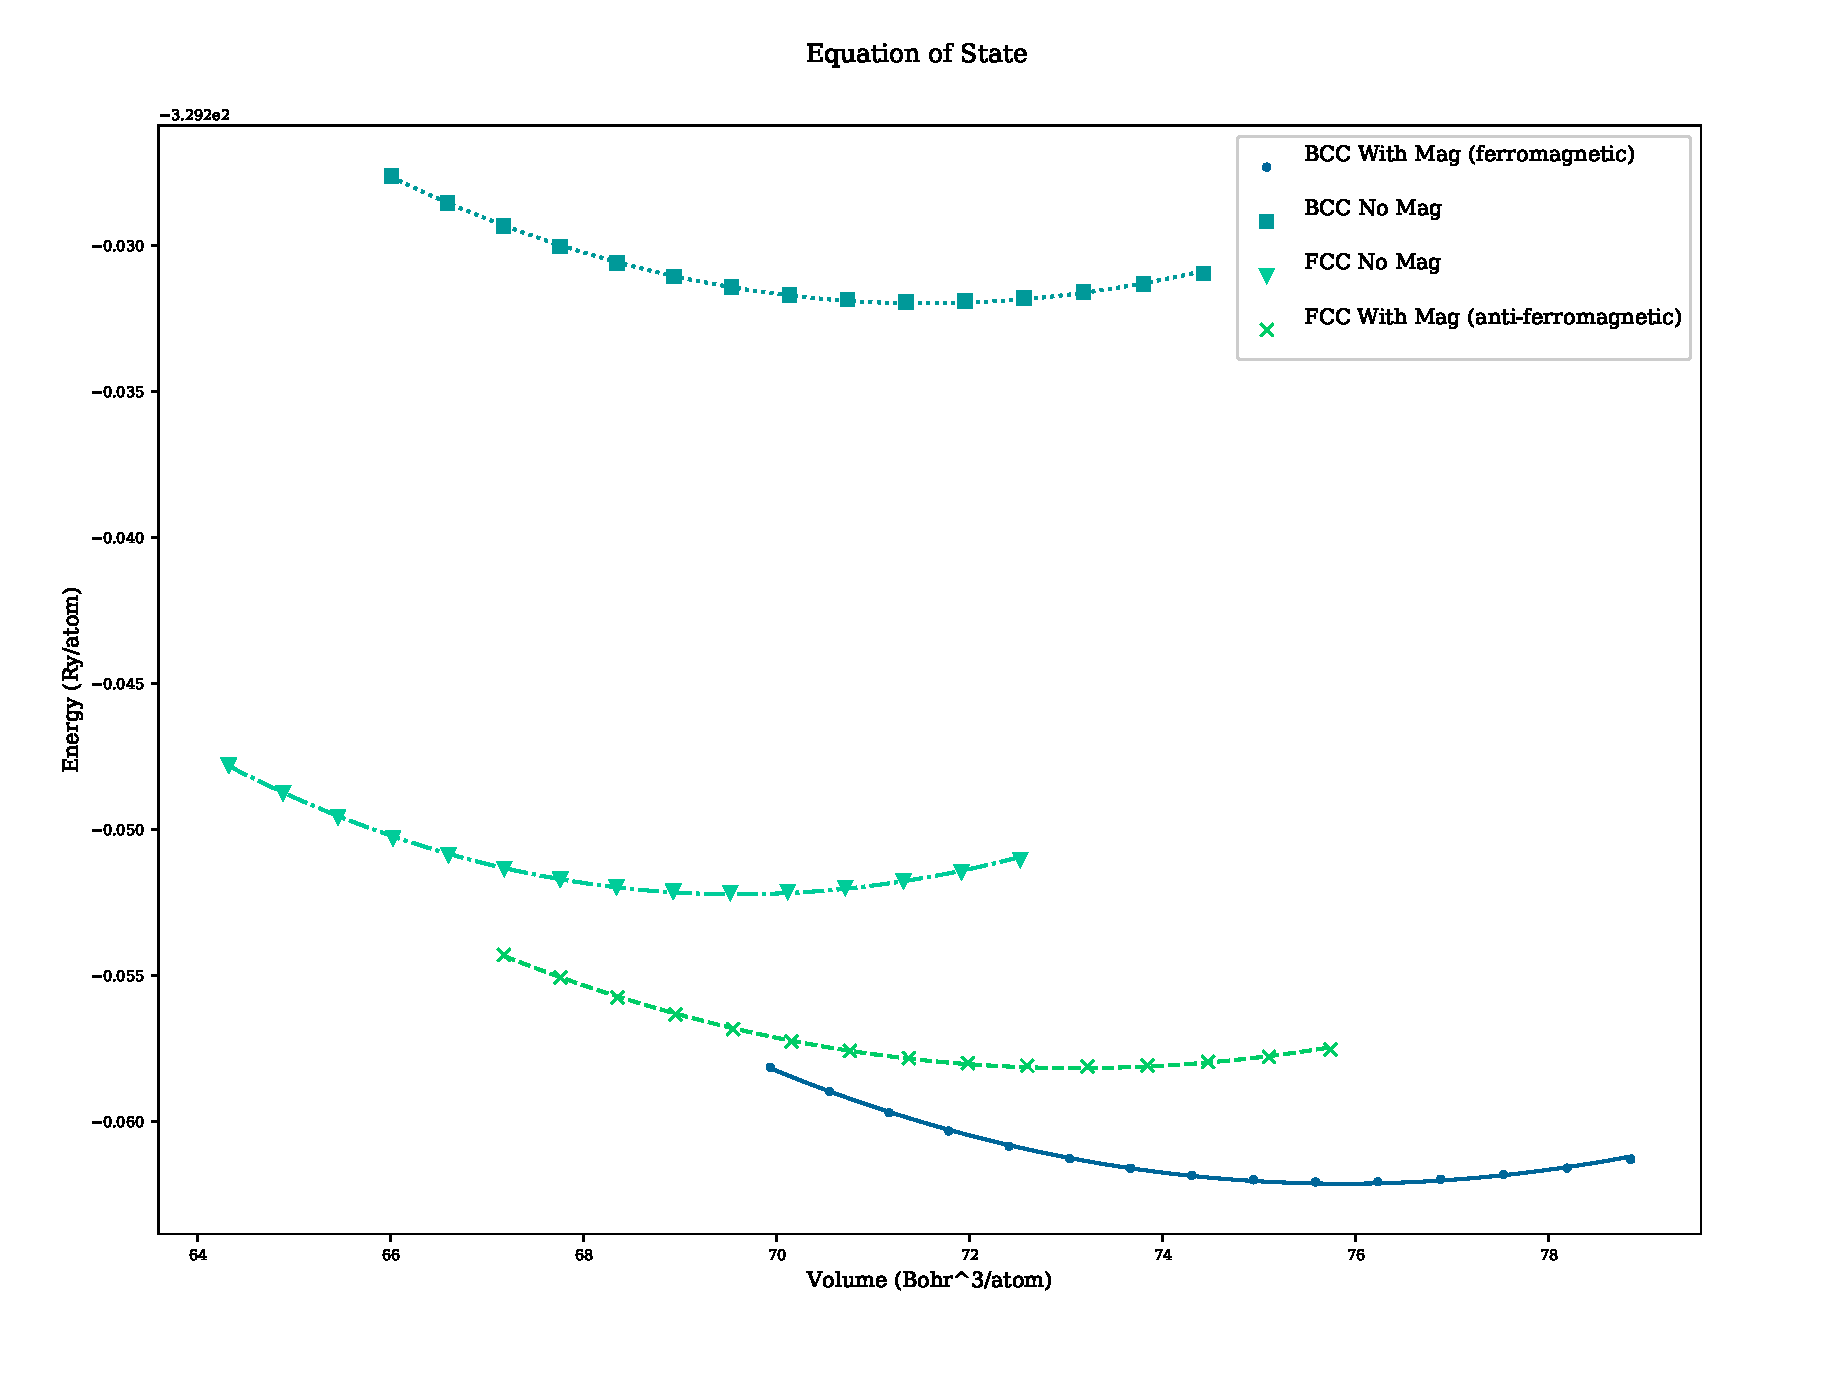
\includegraphics[scale=0.45]{chapters/results_dft_reference_db/qeeos_plots/fe-mag/iron_eos_comparison.eps}
\caption{Equation of state fit through data points for Iron BCC (no magnetism, ferromagnetic) and Iron FCC (no magnetism and antiferromagnetic)}
\end{center}
\label{fig:iron_bcc_fcc_eos}
\end{figure}
\FloatBarrier


\begin{table}[h]
\begin{center}
\renewcommand{\arraystretch}{1.2}
\begin{tabular}{c c c c c c}
\hline\hline
Description & A0 (ang) & V0 ($bohr^3$) & B0 (GPA) & E0 (Ry) (DFT Only) \\
\hline\hline
Exp. & 2.86 & 79.01 & 170 & - \\
No Mag & 2.77 & 71.53 & 286 & -329.23 \\
FM & 2.82 & 75.9 & 239 & -329.26 \\
AFM & (failed) & (failed) & (failed) & (failed) \\
\hline\hline
\end{tabular}
\end{center}
\caption{\acrshort{bcc} Iron properties with and without collinear spin}
\label{table:feproperties}
\end{table}

In the case of Iron, both BCC and FCC configurations were used.  The antiferromagnetic configurations for both BCC and FCC failed in that the SCF calculations failed to converge.  As expected, the optimal configuration was BCC with ferromagnetism, and second to this was FCC with ferromagnetism.

Despite the increase in computational time, and other demands on resources such as scratch space and RAM per node, it was clear that collinear spin calculations were required for iron.  The lattice parameter value was within 2\% of the experimental value with the BCC structure set in a ferromagnetic state.  Whilst the bulk modulus is only within 41\% of the experimental value, this is an improvement over the non magnetic calculation that was almost 70\% away from the experimental bulk modulus (table \ref{table:feproperties}, figure \ref{fig:iron_bcc_fcc_eos}).


\FloatBarrier
\subsection{Convergence Results}

The QECONVERGE program was used to suggest the parameters to use, given the convergence threshold of $1.0 \time 10^{-5} RY/Bohr$ for forces and $1.0 \time 10^{-6} RY$ for energy.

\begin{table}[h]
\begin{center}
\renewcommand{\arraystretch}{1.2}
\begin{tabular}{c c c c c c c}
\hline\hline
Element & Pseudopotential & Ecutwfc & Ecutrho & K-points & Degauss & Atoms\\
\hline\hline
Al & Al PBE KJPAW & 50 & 200 & 11 & 0.04 & 32\\
Fe/Pd/Ru & PBE KJPAW & 71 & 431 & 9 & 0.04 & 32 \\ 
Fe/Pd/Ru & PBE KJPAW & 71 & 431 & Gamma & 0.04 & 128-256 \\ 
\hline\hline
\end{tabular}
\end{center}
\caption{DFT Settings - pseudo-potentials, ecutwfc, ecutrho, k-points, smearing}
\label{table:dftsettingsa}
\end{table}
\FloatBarrier

These settings in table \ref{table:dftsettingsa} were used throughout the remainder of the work.  The maximum values were selected from Fe, Ru and Pd as they were to be used for calculations of the pure elements and for binary allows of Fe-Ru and Fe-Pd.

The other settings used in PWscf throughout are listed in table \ref{table:dftsettingsb}.  Several of these values were arrived at by trial and error.  It was recommended by the authors of Quantum Espresso to adjust parameters such as the mixing beta if a calculation fails to converge.  The mixing mode was also changed from time to time, but overall the plain mode seemed to work best in most cases.

\begin{table}[h]
\begin{center}
\renewcommand{\arraystretch}{1.2}
\begin{tabular}{c c}
\hline\hline
Parameter & Value \\
\hline\hline
etot\_conv\_thr & 0.0001 \\
forc\_conv\_thr & 0.001 \\ 
conv\_thr & $1.0 \times 10^{-8}$ to $1.0 \times 10^{-6}$ \\ 
diagonalization & david \\ 
mixing\_beta & 0.1 to 0.3 \\ 
mixing\_mode & plain (local-TF for defects or randomised configurations) \\ 
\hline\hline
\end{tabular}
\end{center}
\caption{DFT Settings - other settings}
\label{table:dftsettingsb}
\end{table}

\FloatBarrier

The choices of parameters are supported by the convergence plots produced by the QECONVERGE code in figures \ref{image:aluminiumecut} and \ref{image:aluminiumkpointsmearing} (appendix \ref{section:dftconvplots}).




%%%%%%%%%%%%%%%%%%%%%%%%%%%%%%%%%%%%%%%%%%%%%%%%%%%%%%%%%%%%%%%%%%%%%%%%%%%%%%%%%%%%%%%%%%%%%%%%%%%%%%%%%%
%%
%%  Preliminary Calculations
%%  
%%%%%%%%%%%%%%%%%%%%%%%%%%%%%%%%%%%%%%%%%%%%%%%%%%%%%%%%%%%%%%%%%%%%%%%%%%%%%%%%%%%%%%%%%%%%%%%%%%%%%%%%%%


\FloatBarrier
\section{Preliminary Calculations}

\subsection{Relaxed Crystal Calculations}

The cohesive energy is an important value in relation to the interatomic potential.  The energies calculated by \acrshort{dft} code depend on many factors including the energy under which plane-wave are cut-off, the degauss value, k-point settings and the \acrshort{scf} convergence parameters.  What is more important in the \acrshort{dft} calculations is the difference in energy between calculations.  As the cohesive energy is known, a \acrshort{dft} calculation may be performed for each species of atom to determine the relaxed energy.  This value may then be used to calibrate other \acrshort{dft} calculations, so they are given relative to the energy of each atom spaced infinitely far from one another, with a binding energy of 0eV.  The relaxed energies, the settings used to calculate them and the adjustment to convert them to the \enquote{real} energies are given in table \ref{table:relaxedenergies}.

\clearpage
\begin{landscape}

\begin{table}[h]
\begin{center}
\renewcommand{\arraystretch}{1.2}
\begin{tabular}{c c c c c c c}
\hline\hline
Measurement & Al FCC & Fe BCC & Fe FCC & Pd FCC & Ru HCP \\
\hline\hline
Element                    & Aluminium & Iron & Iron & Palladium & Ruthenium & Ruthenium \\
Structure                  & FCC  & BCC  & FCC  & FCC  & HCP  & FCC     \\
Ecutwfc (Ry)               & 50  & 71  & 71  & 71  & 71  & 71    \\
Ecutrho                    & 200 & 430  & 430  & 430 & 430  & 430   \\
K-points                   & 11 11 11 & 9 9 9  & 9 9 9  &  9 9 9  &  9 9 9  &  9 9 9  \\ 
Smearing (Ry)              & 0.04  & 0.04  & 0.04  & 0.04 & 0.04 & 0.04   \\ 
NSpin                      & 0 & 2  & 2  & 0 & 0 & 0  \\ 
Starting Magnetism         & None & FM  & AFM  & None  & None  & None   \\ 
No. Atoms                  & 32  & 16  & 32  & 32 & 16 & 32  \\  
Energy (Ry)                & -1264.08749654  & -5268.18846365   & -10536.25040753    & -16384.95803030  & -6906.78722345  & -13813.30088106  \\
Energy/Atom (Ry)           & -39.502734267   & -329.261778978   & -329.257825235     & -512.029938447 & -431.674201466 & -431.665652533  \\
Energy/Atom (eV)           & -537.462275214  & -4479.836349416  & -4479.782555982    & -6966.524743211   \\
Known Cohesive Energy (eV) & -3.36           & -4.316           & -4.26 (Calculated) & -3.91  & -6.74  & -6.62 (Calculated)             \\
Adjustment/atom (eV)       &  534.102275214  &  4475.520349416  &  4475.520349416    &  6962.614743211 & 5866.47338  &  5866.47338 \\
Relaxed $a_0$ (Bohr)       & 15.265          & 10.594           & 12.937             & 14.845            \\
Relaxed $c$ (Bohr)       & None  & None  & None  & None  & 1.5773  & None \\
$U_{xx}$                   & 1.000           & 1.000            & 1.000              & 1.000              & 1.000            & 1.000           \\
$U_{yy}$                   & 1.000           & 1.000            & 1.054              & 1.000               & 0.8660            & 1.000          \\
$U_{zz}$                   & 1.000           & 1.000            & 1.000              & 1.000                & 1.5773            & 1.000         \\
$U_{yx}$                   & 0.000           & 0.000            & 0.000              & 0.000                & -0.5            & 0.000         \\
\hline\hline
\end{tabular}
\end{center}
\caption{Relaxed energies calculated in Quantum Espresso}
\label{table:relaxedenergies}
\end{table}

\end{landscape}
\clearpage




\subsection{Relaxed FCC Iron}
\label{section:fcc-iron}

The configuration for Fe has been referred to throughout this work as \acrshort{fcc}, but the relaxed collinear spin-polarized \acrshort{dft} calculation predicts that the structure is slightly \acrfull{fct}.  The optimal magnetic setting is antiferromagnetic (fig. \ref{graph:iron_bcc_fcc_eos}) and, with the spin aligned in the z-direction, the y-axis of the unit cell is approximately 5\% larger than the x and z axis.

\begin{figure}[ht] 
  \begin{minipage}[b]{0.8\linewidth}
    \centering
    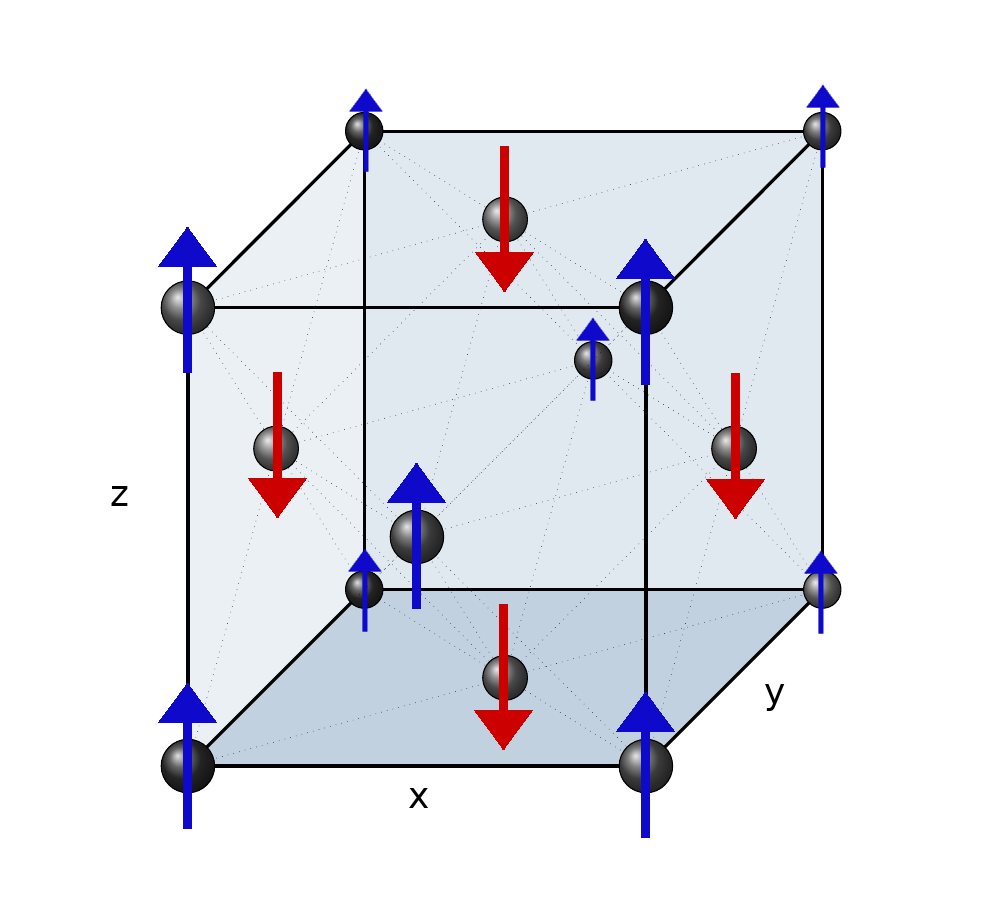
\includegraphics[width=.9\linewidth]{chapters/results_dft_reference_db/images/fe-austenitic-mag.png} 
    \caption{Magnetic alignment along the z-axis, antiferromagnetic Fe fcc}  
  \end{minipage}
  \label{fig:ironfccantiferromagnetic}
\end{figure}

The atoms in the (0,1,0) plane are majority spin-up electrons, along the z-axis, and those in the (0,2,0) plane are spin-down, along the z-axis (fig. \ref{fig:ironfccantiferromagnetic}).  Following the relaxation calculation, all the atoms were in their standard \acrshort{fcc} positions, and the magnetic moment for each atom was 1.4901 \gls{bohrmagneton} and -1.4901 \gls{bohrmagneton} for the spin up and down respectively.  





%% 13.6056980659

%%%%%%%%%%%%%%%%%%%%%%%%%%%%%%%%%%%%%%%%%%%%%%%%%%%%%%%%%%%%%%%%%%%%%%%%%%%%%%%%%%%%%%%%%%%%%%%%%%%%%%%%%%
%%
%%  QEEOS
%%  
%%%%%%%%%%%%%%%%%%%%%%%%%%%%%%%%%%%%%%%%%%%%%%%%%%%%%%%%%%%%%%%%%%%%%%%%%%%%%%%%%%%%%%%%%%%%%%%%%%%%%%%%%%


\FloatBarrier
\section{QEEOS Python Code}
\label{code:qeeos}

\FloatBarrier
\subsection{Purpose of Code}

A code was developed to automate the process of calculating the equation of state and elastic constants of a material using Quantum Espresso.  It requires an input file and a starting PWscf input file.  

\begin{itemize}
\item the input configuration is relaxed using the vc-relax option in PWscf
\item configuration files are created to compute the equation of state, and PWscf is used to calculate the energies of these configurations
\item to compute the elastic constants, nine distortions are applied to the relaxed configuration with the required number of steps for each strain applied to each distortion, and these are processed with PWscf
\item once all \acrshort{dft} work has completed, the Birch-Murnaghan equation of state is fit to the first set of energies, and the nine orthorhombic elastic constants are fit to the results of the second set of energies
\end{itemize}


\FloatBarrier
\subsection{Source Code and Instructions}

The source code and instructions on how to use the program are available to download from GitHub.

https://github.com/BenPalmer1983/qe\_eos




%%%%%%%%%%%%%%%%%%%%%%%%%%%%%%%%%%%%%%%%%%%%%%%%%%%%%%%%%%%%%%%%%%%%%%%%%%%%%%%%%%%%%%%%%%%%%%%%%%%%%%%%%%
%%
%%  ELASTIC PROPERTIES
%%  
%%%%%%%%%%%%%%%%%%%%%%%%%%%%%%%%%%%%%%%%%%%%%%%%%%%%%%%%%%%%%%%%%%%%%%%%%%%%%%%%%%%%%%%%%%%%%%%%%%%%%%%%%%

\FloatBarrier
\section{Calculated Elastic Properties}
\label{section:resultselastic}

The planewave cutoff and k-points were converged to within the required parameters for energy and force but it is known that, in general, \acrshort{lda} and \acrshort{gga} pseudopotentials under and over estimate the lattice parameters.  The bulk modulus and elastic constants were calculated for \acrshort{fcc} Aluminium and \acrshort{bcc} Iron in order to compare to experimental values.

A summary of the main data points is given here for \acrshort{fcc} Al, \acrshort{bcc} Fe, \acrshort{fcc} Pd and \acrshort{fcc} Fe, and the first three listed are compared to experimental data.  A full details of the calculated properties including plots are included in appendix \ref{chapter:dftcalculatedproperties}.

\subsection{FCC Aluminium}

The parameters used for the Al calculations were arrived at earlier using the convergence code.  The remainder of the parameters are either default settings, or were selected following trial and error (for example, reducing the mixing beta to help achieve convergence).  These settings are given in table \ref{table:alfccdftsettings}.






The results in table \ref{table:alfccexperimentaldft} show a good agreement between the experimental values for Al and the calculated values.  The lattice parameter is a particularly good fit, being within 1\% of the experimental value.  The shear modulus does not match as well, but is within 20\% of the experimental value.  The \acrshort{rss} measurement of fit between the values was $2.54 \times 10^2$.



\FloatBarrier
\subsection{BCC Iron}

The equation of state and elastic constants were calculated for \acrshort{bcc} Fe, with no-spin and collinear spin.  The settings used for the calculations are given in table \ref{table:febccdftsettings}. 


The non-magnetic Iron calculation was particularly poor.  Although the lattice parameter was within 5\% of the experimental value, the structure was unstable and had negative values for both the Young's modulus and shear modulus (table \ref{table:febccexperimentaldft}).  The \acrshort{rss} measurement of fit between the values for the was $2.01 \times 10^5$.

With collinear spin enabled, the structure is stable.  The lattice parameter is still slightly under the experimental, but is now within almost 2\% of the value.  The bulk modulus predicted by fitting the Birch-Murnaghan equation of state is more than 40\% the experimental value, but the Reuss and Voigt values derived from the calculated elastic constants are just 20\% difference to the experimental value.  The latter two values are calculated using the elastic constants, rather than the equation of state.  This highlights the importance of using collinear spin calculations, despite the cost in computing time.  The \acrshort{rss} measurement of fit between the values was $1.09 \times 10^4$ giving an improvement of at least one magnitude.




\FloatBarrier
\subsection{FCC Iron}
\label{section:fccferesults}

The gamma phase of pure iron does not exist for experimental measurements to be made, and the results here will be used to fit the FCC iron potential in chapter \ref{chap:resultsfitting}.  The settings used for the calculations are given in table \ref{table:fefccdftsettings}. 

The structure is stable under the orthorhombic stability conditions given in section \ref{section:stabilityconditions}.  Whilst there are no experimental measurements to check against, the values are sane when compared to the other calculations performed here (table \ref{table:fefccexperimentaldft}).  The $C_{44}$, $C_{55}$ and $C_{66}$ values are slightly large when compared with those for \acrshort{bcc}, but further \acrshort{dft} calculations would need to be performed to investigate this.  

\begin{table}[ht]
\renewcommand{\arraystretch}{1.2}
\begin{tabular}{lccc}
\hline\hline
Property & \multicolumn{3}{c}{Value used in potential fitting} \\
\hline\hline
Element & \multicolumn{3}{c}{Fe}\\
Structure             & \multicolumn{3}{c}{Face Centered Cubic}\\
$a_0$                 & \multicolumn{3}{c}{3.59 Angstrom}\\
Nearest Neighbour     & \multicolumn{3}{c}{1.85 Angstrom}\\
Basis vectors         & $\begin{bmatrix} 0.96 & 0.0 & 0.0 \\ 0.0 & 1.00 & 0.0 \\ 0.0 & 0.0 & 0.96  \end{bmatrix}$ \\
$E_{coh}$             & \multicolumn{3}{c}{-4.32 eV}   \\
$B_0$ (GPA)           & \multicolumn{3}{c}{226.1}   \\
$E$ (GPA)             & \multicolumn{3}{c}{356.8}   \\
$G$ (GPA)             & \multicolumn{3}{c}{144.8}   \\
Poisson Ratio $\eta$  & \multicolumn{3}{c}{0.23}   \\
Elastic Constants     & $\begin{bmatrix} 364.6 & 141.6 & 233.8 & 0 & 0 & 0 \\ 141.6 & 298.7 & 130.4 & 0 & 0 & 0 \\ 233.8 & 130.4 & 364.6 & 0 & 0 & 0 \\ 0 & 0 & 0 & 186.3 & 0 & 0 \\ 0 & 0 & 0 & 0 & 266.8 & 0 \\ 0 & 0 & 0 & 0 & 0 & 186.3 \end{bmatrix}$ \\
\hline\hline
\end{tabular}
\caption{Fe input parameters for fitting}
\label{table:feinputparameters}
\end{table}








\FloatBarrier
\subsection{FCC Palladium}

The equation of state and elastic constants were calculated for \acrshort{fcc} Pd with no-spin.  The settings used for the calculations are given in table \ref{table:pdfccdftsettings}. 

There is a good agreement between the computed and experimental values for Pd, without the need to move from non-spin to collinear spin calculations (table \ref{table:pdexperimentaldft}).  However, in the alloy calculations the  presence of Fe will dictate the necessity for collinear spin.  The \acrshort{rss} measurement of fit between the values was $4.12 \times 10^3$.

\begin{table}[ht]
\renewcommand{\arraystretch}{1.2}
\begin{tabular}{lccc}
\hline\hline
Property & \multicolumn{3}{c}{Value used in potential fitting} \\
\hline\hline
Element & \multicolumn{3}{c}{PD}\\
Structure             & \multicolumn{3}{c}{Face Centered Cubic}\\
$a_0$                 & \multicolumn{3}{c}{3.925 Angstrom \cite{webelementspd}}\\
Nearest Neighbour     & \multicolumn{3}{c}{ Angstrom \cite{webelementspd}}\\
Basis vectors         & $\begin{bmatrix} 1.0 & 0.0 & 0.0 \\ 0.0 & 1.0 & 0.0 \\ 0.0 & 0.0 & 1.0  \end{bmatrix}$ \\
$E_{coh}$             & \multicolumn{3}{c}{3.91 eV \cite{semiempiricalpots}}   \\
$B_0$                 & \multicolumn{3}{c}{184.4 GPA \cite{semiempiricalpots}}   \\
Elastic Constants     & $\begin{bmatrix} 218.5 & 151.4 & 151.4 & 0 & 0 & 0 \\ 151.4 & 218.5 & 151.4 & 0 & 0 & 0 \\ 151.4 & 151.4 & 218.5 & 0 & 0 & 0 \\ 0 & 0 & 0 & 80.3 & 0 & 0 \\ 0 & 0 & 0 & 0 & 80.3 & 0 \\ 0 & 0 & 0 & 0 & 0 & 80.3 \end{bmatrix}$ \\
\hline\hline
\end{tabular}
\caption{Pd input parameters for fitting}
\label{table:pdinputparameters}
\end{table}





\FloatBarrier
\subsection{FCC Ruthenium}
\label{section:fccferesults}


Ruthenium at standard conditions exists as \acrlong{hcp}, but as this work is focused on \acrshort{fcc} steel doped with \acrshort{pgm}s, the properties are computed for \acrshort{fcc} Ruthenium.  The settings used for the calculations are given in table \ref{table:rufccdftsettings}. 



\begin{table}[ht]
\renewcommand{\arraystretch}{1.2}
\begin{tabular}{lccc}
\hline\hline
Property & \multicolumn{3}{c}{Value used in potential fitting} \\
\hline\hline
Element & \multicolumn{3}{c}{RU}\\
Structure             & \multicolumn{3}{c}{Face Centered Cubic}\\
$a_0$                 & \multicolumn{3}{c}{3.809 Angstrom \cite{webelementspd}}\\
Nearest Neighbour     & \multicolumn{3}{c}{ Angstrom \cite{webelementspd}}\\
Basis vectors         & $\begin{bmatrix} 1.0 & 0.0 & 0.0 \\ 0.0 & 1.0 & 0.0 \\ 0.0 & 0.0 & 1.0  \end{bmatrix}$ \\
$E_{coh}$             & \multicolumn{3}{c}{6.624 eV \cite{semiempiricalpots}}   \\
$B_0$                 & \multicolumn{3}{c}{307.8 GPA \cite{semiempiricalpots}}   \\
Elastic Constants     & $\begin{bmatrix} 471.5 & 219.1 & 219.1 & 0 & 0 & 0 \\ 219.1 & 471.5 & 219.1 & 0 & 0 & 0 \\ 219.1 & 219.1 & 471.5 & 0 & 0 & 0 \\ 0 & 0 & 0 & 245.0 & 0 & 0 \\ 0 & 0 & 0 & 0 & 245.0 & 0 \\ 0 & 0 & 0 & 0 & 0 & 245.0 \end{bmatrix}$ \\
\hline\hline
\end{tabular}
\caption{Pd input parameters for fitting}
\label{table:ruinputparameters}
\end{table}






%%%%%%%%%%%%%%%%%%%%%%%%%%%%%%%%%%%%%%%%%%%%%%%%%%%%%%%%%%%%%%%%%%%%%%%%%%%%%%%%%%%%%%%%%%%%%%%%%%%%%%%%%%
%%
%%  Results DFT Database
%%  
%%%%%%%%%%%%%%%%%%%%%%%%%%%%%%%%%%%%%%%%%%%%%%%%%%%%%%%%%%%%%%%%%%%%%%%%%%%%%%%%%%%%%%%%%%%%%%%%%%%%%%%%%%




\FloatBarrier
\section{DFT Configuration Database}
\label{section:dftconfigurationdbresults}


\subsection{Calibrating the Cohesive Energies}

The isolated and relaxed energy values were computed and from these values the cohesive energies were calculated (figure \ref{fig:isolatedatoms} and table \ref{table:calculatedcohesiveenergies}).  In doing so, it became apparent that there were errors of up to 12\% between the known values and those computed with \acrshort{dft}.

\begin{figure}[h]
\begin{center}
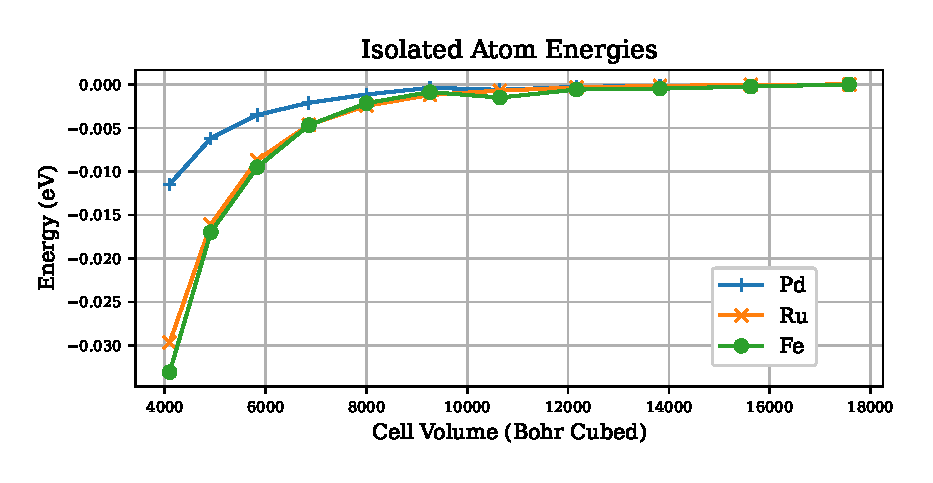
\includegraphics[width=0.5\linewidth]{chapters/results_dft_reference_db/isolated/isolated_63.eps}
\caption{Isolated atom energies as cell size increase}
\label{fig:isolatedatoms}
\end{center}
\end{figure}

An offset was needed to convert from the \acrshort{dft} energies to \enquote{real} energies that could be used to derive a potential.

\begin{table}[h]
\begin{center}
\begin{tabular}{c c c c c}
\hline\hline
Element & Structure & Isolated Energy (Ry) & Relaxed Energy (Ry) & Cohesive Energy (eV) \\
\hline\hline
Fe      & BCC       & -4474.99115          & -4479.83524         & 4.84 (exp. 4.32)\\
Fe      & FCC       & -4474.99115          & -4479.78095         & 4.79 \\
Pd      & FCC       & -6962.47261          & -6966.52234         & 4.05 (exp. 3.91)\\
Ru      & HCP       & -5866.39894          & -5873.22666         & 6.83 (exp. 6.74)\\
Ru      & FCC       & -5866.39894          & -5873.11029         & 6.71 \\
\hline\hline
\end{tabular}
\end{center}
\caption{\acrshort{dft} calculated energies per atom}
\label{table:calculatedcohesiveenergies}
\end{table}

Two offsets were computed and these depend upon the settings used in the calculation (table \ref{table:calculatedoffset}).  Specifically, they depend on whether 9x9x9 k-points are used, in the case of the 32 atom calculations, or the gamma point is used (128, 129 and 256 atoms).

\begin{table}[h]
\begin{center}
\begin{tabular}{c c c c c}
\hline\hline
Element & Reference Structure & Energy (Ry) (9x9x9) & Energy (Ry) (Gamma) & Cohesive (eV)\\
\hline\hline
Fe      & BCC  & -329.2618197  & -84290.00709480 & -4.316 \\
Pd      & FCC  & -512.0299524  & -131079.09207327 & -3.91 \\
Ru      & HCP  & -431.6742014  & -110507.45936537 & -6.74 \\
\hline\hline
\end{tabular}
\end{center}
\caption{Relaxed energies for 32 atoms, using 9x9x9 k-points, and 256 atoms, using the gamma point.  These were used with the known cohesive energy to compute the offset energy.}
\label{table:calculatedoffset}
\end{table}



\subsection{Complete DFT Reference Database}

The complete database of configurations was compiled from many of the already mentioned calculations.  The QEEOS code that computed the bulk properties creates PWscf input files and processes the output files.  These output files are saved but the program and are as valid to use in the reference database as any.  In total the database has over 600 configurations for Fe-Pd and almost 600 for Fe-Ru.  

\begin{figure}
\begin{subfigure}{.32\textwidth}
  \centering
  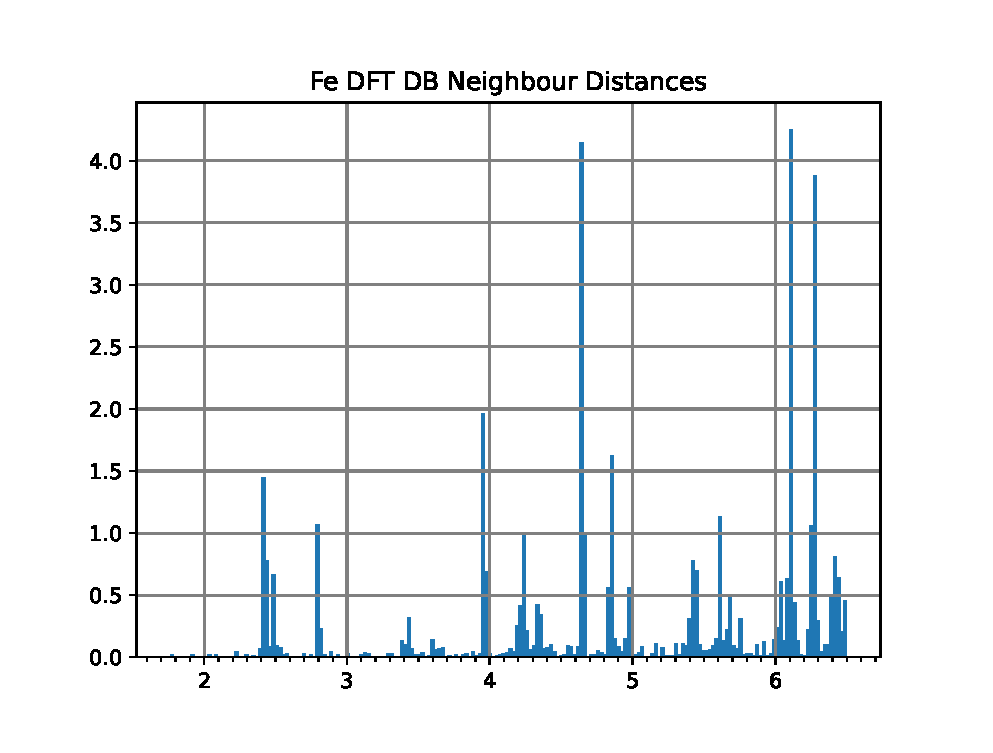
\includegraphics[width=.94\linewidth]{chapters/results_dft_reference_db/neighbour_distances/db_fe_neighbours.eps}  
  \caption{Single atom, 256 atoms in total}
  \label{fig:sub-first}
\end{subfigure}
\begin{subfigure}{.32\textwidth}
  \centering
  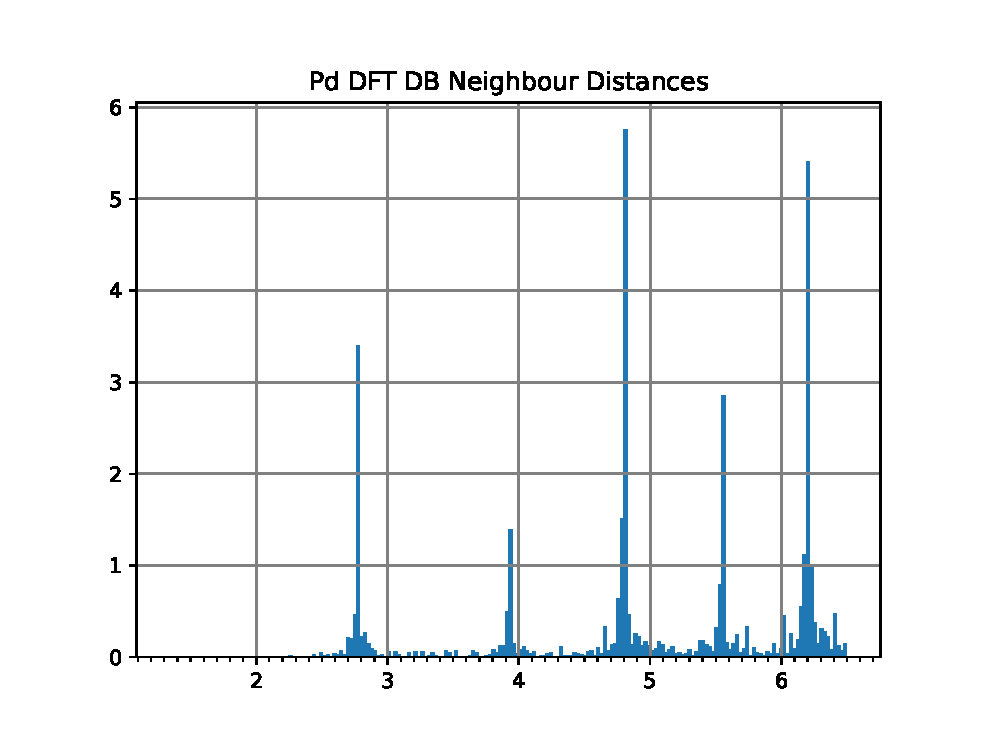
\includegraphics[width=.94\linewidth]{chapters/results_dft_reference_db/neighbour_distances/db_pd_neighbours.eps}  
  \caption{Multiple atoms, 256 atoms in total}
  \label{fig:sub-first}
\end{subfigure}
\begin{subfigure}{.32\textwidth}
  \centering
  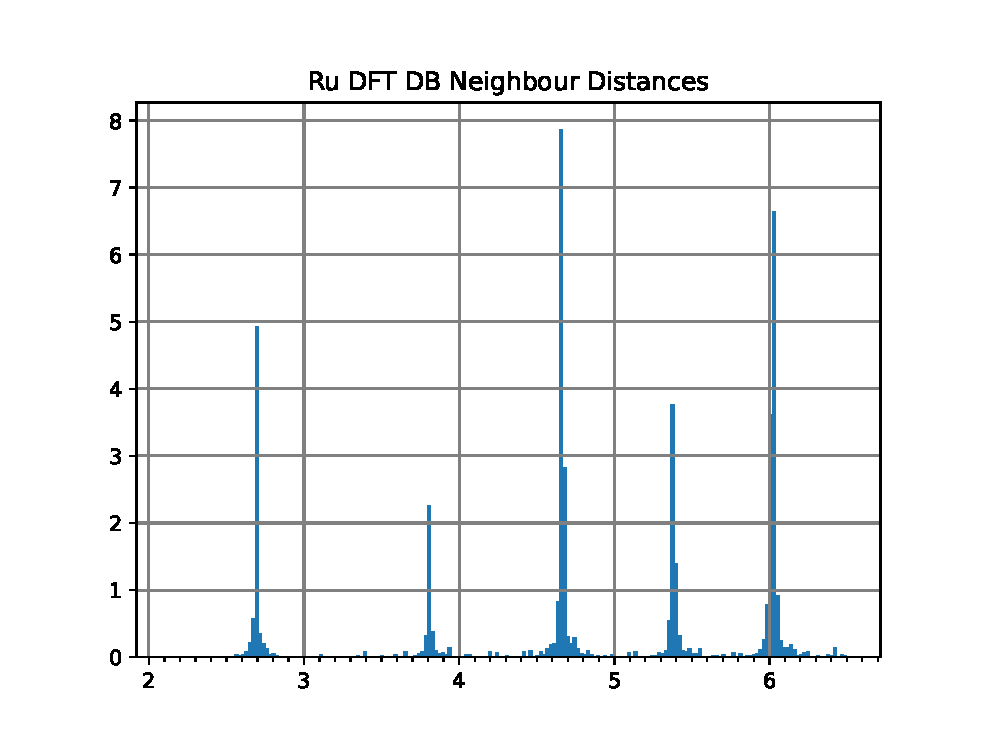
\includegraphics[width=.94\linewidth]{chapters/results_dft_reference_db/neighbour_distances/db_ru_neighbours.eps}  
  \caption{Multiple atoms, 256 atoms in total}
  \label{fig:sub-first}
\end{subfigure}
\begin{subfigure}{.32\textwidth}
  \centering
  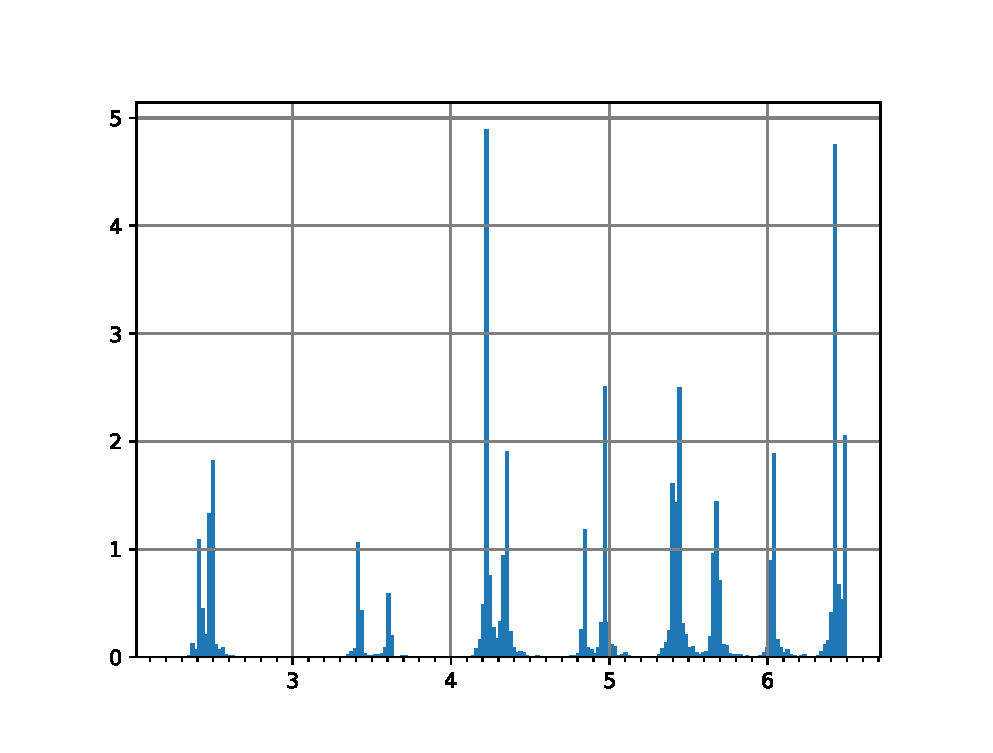
\includegraphics[width=.94\linewidth]{chapters/results_dft_reference_db/neighbour_distances/db_fepd_neighbours.eps}  
  \caption{Multiple atoms, 256 atoms in total}
  \label{fig:sub-first}
\end{subfigure}
\begin{subfigure}{.32\textwidth}
  \centering
  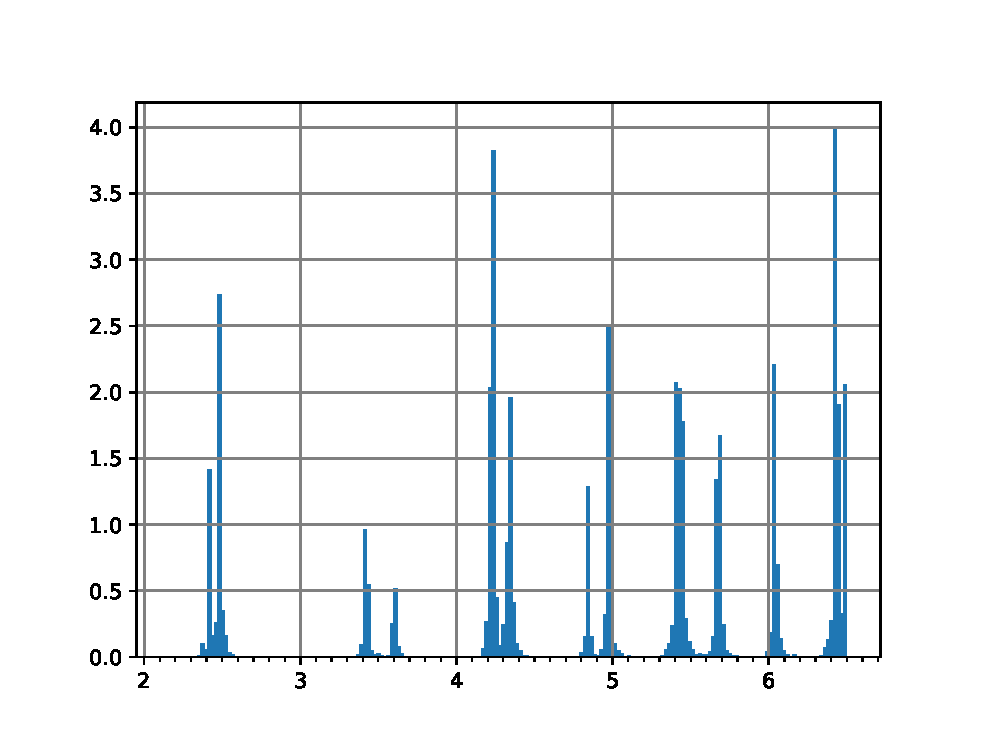
\includegraphics[width=.94\linewidth]{chapters/results_dft_reference_db/neighbour_distances/db_feru_neighbours.eps}  
  \caption{Multiple atoms, 256 atoms in total}
  \label{fig:sub-first}
\end{subfigure}
\label{fig:dbneighbourseparations}
\end{figure}

The distribution of atom separations was measured across the database and these are plotted in figure \ref{fig:dbneighbourseparations}.  The full set is available to download from https://github.com/BenPalmer1983/fepd\_feru\_potential.













